\documentclass[11pt]{exam}
\usepackage{commonheader}
\usepackage{graphicx}
\graphicspath{ {./images/sus.png} }

% Use the following to toggle solutions/metas
\printsolutions % uncomment me
% \printmeta % uncomment  me

\discnumber{8}
\title{Red Black Trees \& Heaps}
\date{October 12 - 14, 2022}

\begin{document}
\maketitle

%%%%%%%%%%%%%%%%%%%%%%%%%%%%%%%
% RB Trees % 
%%%%%%%%%%%%%%%%%%%%%%%%%%%%%%%

\section{Black Diamond Crepe Myrtle}
\begin{questions}
\subimport{topics/trees/balanced-search-trees/medium/}{llrb-psuedo.tex}
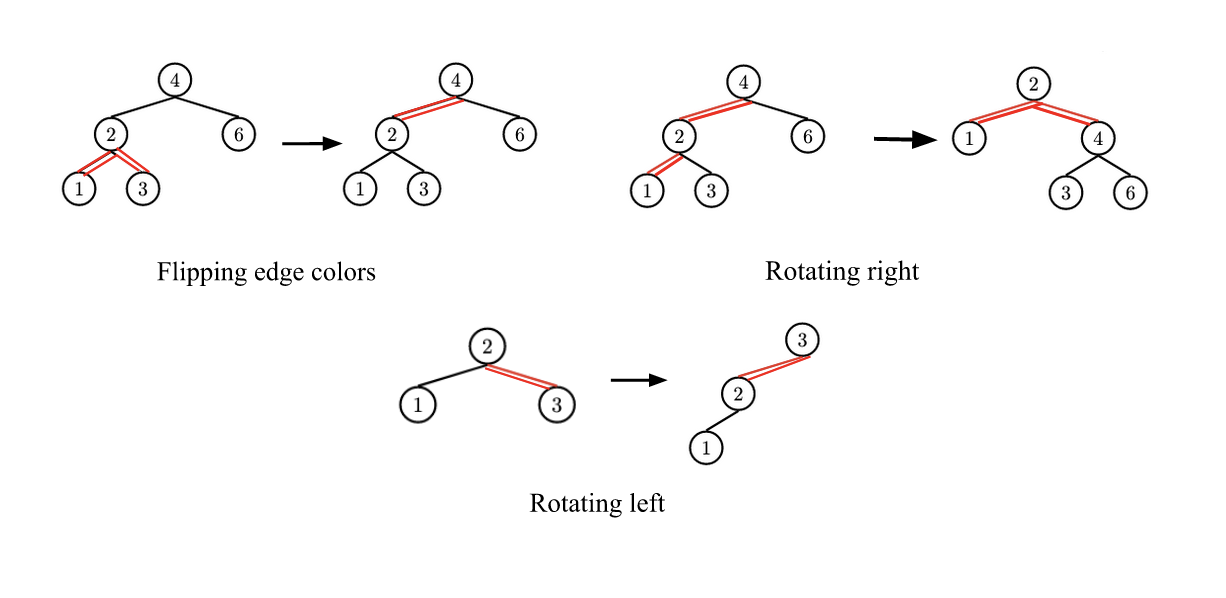
\includegraphics[scale=.8]{images/llrb_examples.png}
\clearpage
\subimport{topics/trees/balanced-search-trees/medium/}{llrb-hug.tex}
\end{questions}

%%%%%%%%%%%%%%%%%%%%%%%%%%%%%
% Hashing (Implementation) %
%%%%%%%%%%%%%%%%%%%%%%%%%%%%%

\pagebreak
\section{HashTables (ft. CSM Content Staff)}
\begin{questions}
\subimport{topics/hashing/medium/}{hashing_implementation.tex}

\includegraphics[scale=.025]{images/sus.png}
\end{questions}

%%%%%%%%%%%%%%%%%%
% Hashing Runtimes %
%%%%%%%%%%%%%%%%%%

\pagebreak
\section{Hashing Runtimes}
\begin{questions}
\subimport{topics/hashing/easy/}{motivation.tex}
\end{questions}


%%%%%%%%%%%%%%%
% Priority Queue: Min-Heap %
%%%%%%%%%%%%%%%

\pagebreak
\section{Chonky Slimes}
\begin{questions}
\subimport{topics/heaps/easy/}{slime-intro.tex}
\subimport{topics/heaps/easy/}{slime-add.tex}
\subimport{topics/heaps/easy/}{slime-remove.tex}
\end{questions}

\end{document}

